\chapter{Ejemplo de capítulo de resultados}


\section{Sección}

Las tablas se pueden referenciar como: en la \autoref{tab:comp} se muestran valores.

\begin{table}[h!]
\centering
\caption{Descripción de tabla.}
\label{tab:comp}
\begin{tabular}{|c|c|c|}
  \hline
  $t$ (seg) & $x$(t) & $y$(t)\\
  \hline
  1 & 0.0000 & 0.0001\\
  2 & 0.5000 & 0.2498\\
  3 & 1.0000 & 1.0000\\
  4 & 1.5000 & 2.2403\\
  5 & 2.0000 & 4.0010\\
  6 & 2.5000 & 6.2459\\
  \hline
\end{tabular}
\end{table}

También se pueden referenciar las figuras como la \autoref{fig:comp}.

\begin{figure}[h!]
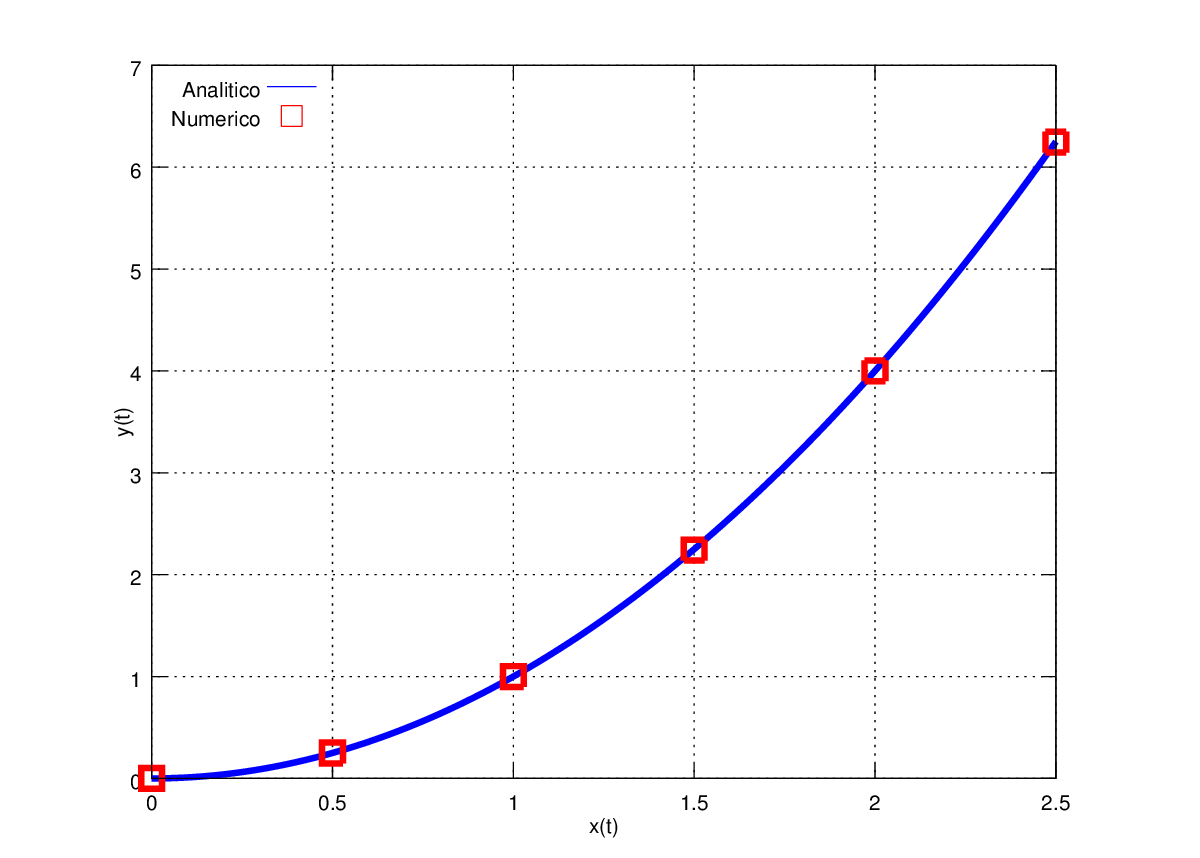
\includegraphics[width=\textwidth]{imagenes/chap4/x_vs_y}
\caption{Descripción de figura, también se deben incluir referencias si la imagen no fue creada por los autores \citep{LeMagorou2002}.}
\label{fig:comp}
\end{figure}

Esto es un ejemplo de ecuación... ver Ecuación~\eqref{eqn:ref}.
\begin{equation}\label{eqn:ref}
\dot{w} = \int_0^T \int_{\Omega} \sigma(t) : \dot{\varepsilon}(t) \, dV \, dt
\end{equation}


También se pueden referenciar otras secciones de la tesina como el \autoref{sec2}, o la \autoref{subsec}, que se encuentra en la página \pageref{sec2}.